\chapter{Optimization of the cross section for power extraction}
\label{chap:cross-sections}
\section{Introduction}

%Galloping occurs as a result of the pressure difference created due to the relative distance between the shear layers and the respective walls of the cross section, at the top and bottom sides of the body. As discussed in section \ref{subsec:c_y and shear layers}, the instantaneous induced angle makes one of the separated shear layers closer to the wall creating a low pressure region. This pressure difference results in a transverse forcing (normal to the direction of the flow) which becomes in phase with the transverse velocity and sustains galloping.  JL: this needs to be re-written. Even I don't really know what you are trying to say here. I think you are mixing up a description of the flow, and the hypothesis that you are going to test.


 Galloping is due to an increase in mean induced lift force \cy\  with an increase in the instantaneous induced angle of attack. This instantaneous angle of attack is directly related to the transverse velocity - an increase in angle of attack implies an increase in velocity. This increase in mean lift force is created by an increase in the difference in mean pressure on the upper and lower sides of the body. The mean pressure on each side of the body is related to the structure of the mean shear layer, in particular to the separation and potential reattachment of this shear layer, and the size of any resulting recirculation region. An increase in angle of attack forces one shear layer (the lower one in figure \ref{fig:shear-layer-sketch}) closer to the wall, meaning a high speed region is placed close to this wall. A simple consideration of Bernoulli's equation shows that this high speed region should result in a region of low pressure. This low pressure on the upper side results in a positive pressure difference between the lower and upper sides, and thus a positive mean lift. The fact that this mean lift occurs as a function of the angle of attack, and therefore the transverse velocity, implies that this transverse forcing should be in phase with the transverse velocity.

From equation \ref{eqn:power_alt} discussed in section \ref{subsec:ave_pow} it is clear that the power transferred from fluid to the body is a function of the induced forcing $F_y$ and the transverse velocity $\dot{y}$. The sign of the average power represents the direction of power transfer; positive power represents the power transfer from fluid to the body, negative power represents power transferring from body to the fluid. Thus, according to equation \ref{eqn:power_alt} it can be deduced that if there is a scenario where both high induced forcing and high transverse velocities are present, higher power output can be achieved.

This can be related directly to the shape of the $C_y$ vs. $\theta$ curve. To optimize power
transfer this curve should,

\begin{itemize}
\item have a high gradient $\partial C_y/\partial \theta$ at
  $\theta = 0$
\item a large maximum $C_y$
\item this maximum $C_y$ should occur at a high value of $\theta$
\end{itemize}

All of these features can be influenced by the cross section of the
body which is galloping. Therefore, if the geometric features of the
cross section that influence these curve features can be identified,
an informed search for an optimal cross section for power extraction
can be undertaken. The major features of the body that influence these
$C_y$ vs. $\theta$ curve parameters are discussed below.

\citet{Luo1994}, showed that the afterbody of the cross section has a direct impact on the $C_y$ vs. $\theta$ curve. One interesting observation of this study was that inhibiting the shear layer re-attachment results in a higher peak induced force coefficient $C_y$ occurring at high induced angles (high transverse velocities). The opposite of this result was discussed by \citet{Robertson2003} where long rectangular cross sections did not exhibit galloping due to shear layer reattachment at low $\theta$. Furthermore, \citet{Luo1994} have discussed the impact of the reattachment of the shear layer at the trailing edge. As $\theta$ is further increased beyond the angle at which reattachment occurs, the enclosed ``bubble'' region of the separated reattached shear layer shrinks in size reducing the difference in suction in the top and bottom sides of the body and results in a reduction in \cy\ (refer section \ref{subsec:c_y and shear layers}). 

Therefore, it can be hypothesised that a higher power transfer can be obtained by inhibiting the shear layer re-attachment. 

Here, the influence of the shear layer and its reattachment on the mean power is discussed. It is crucial to keep the shear layer closer to the body for galloping; if it moves too far from the body, the relationship between a separated shear layer inducing a high velocity, and therefore low pressure, is lost. Thus, a cross section which has a straight initial section (which provides some initial streamlining) followed by a slanting section to inhibit the shear layer, had to be considered for analysis. Therefore, a cross section which is a hybrid of a rectangle and a triangle is considered, as illustrated in figure \ref{fig:hybrid_section}. This cross section was essentially developed by slating the afterbody of the square section as illustrated in figure \ref{fig:hybrid_section}. The cross section is transformed gradually by manipulating the ratio of two lengths, the first being the length of the straight section, and the second being the streamwise length of the entire body. This cross section provides the flexibility of gradually inhibiting the shear layer reattachment while having the initial streamlining of the shear layers to keep the shear layers reasonably close to the body to sustain galloping. 

The DNS data for both stationary and FSI cases were obtained at $\reynoldsnumber=200$. The force data are presented for each stationary cross section. This is followed by presentation of extracted power curves, calculate from the QSS model using this force data for each new body. Based on the QSS power data, an optimum cross section for power extraction, from the family of cross sections that have been tested, is identified.

The main features of the generated $C_y$ vs. $\theta$ curves for the
new bodies are identified and linked to the flow structure present by
analysing the mean surface pressure and flow velocity data. Following
this, a comparison is made between QSS and DNS mean power on the cross
section which provides an optimum mean power.

A final summary is presented outlining that the behaviour of the shear layers is a controlling factor for mean power output. The preliminary design considerations to obtain an optimum power output should therefore focus on the manipulation of these shear layers. 





\section{Influence of the shear layers}

In a typical cross section which sustains galloping, the induced lift \cy\ increases with increasing induced angle $\theta$ until it reaches a maximum value of \cy\ where the shear layer reattachment occurs. The lift force then decreases as $\theta$ is further increased. The underlying mechanism for this behaviour is discussed in detail in section \ref{subsec:c_y and shear layers}.   

\subsection*{Selection of the cross section}

\begin{figure}
\setlength{\unitlength}{\textwidth}

  \begin{picture}(1,0.23)(0,0.74)
    
  \put(0.2,0.76){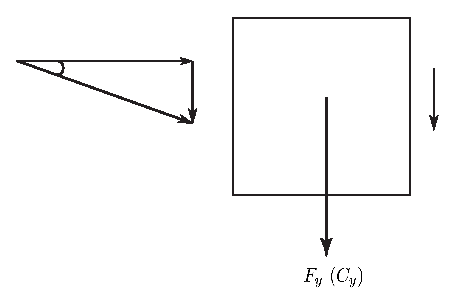
\includegraphics[width=0.5\unitlength]{../FnP/gnuplot/setup-1.eps}}         
      
      
   
 	\put(0.315,0.93){$U$}
 	\put(0.3,0.84){$U_i$}
    \put(0.42,0.88){$\dot{y}$}
    \put(0.28,0.895){ $\theta$}
    \put(0.7,0.87){\small $(+)$}
      	

 	
 	 

     

  \end{picture}

 \caption{Induced angle of attack on the square prism due to the resultant of free-stream velocity of the fluid and transverse velocity of the body.}
    \label{fig:setup_1}
\end{figure}

Several key factors have been considered leading to the selection of a suitable cross section for this analysis. These key factors are:

\begin{itemize}
\item The cross section should have a bluff front face with sharp upstream corners for the flow to separate at the leading edges;

\item As the proximity of shear layers to the body plays a vital role in creating \cy\ \citep{Parkinson1989}, the cross section should have a basic level of streamlining.

\item The cross section should consist of a geometric profile in the afterbody, to inhibit or delay the shear layer reattachment.   
\end{itemize}

The square cross section which is considered as the base cross section in this study satisfies the first two criteria of the selection process. Therefore, in order to inhibit the shear layer reattachment, the top and bottom sides of the trailing edges of the square are tapered off and a hybrid cross section of a rectangle and a triangle (illustrated in figure \ref{fig:hybrid_section}), i.e, a pentagon is produced. This cross section satisfies all criteria in the cross section selection process. Another advantage of this cross section is the inhibition of the shear layer can be varied systematically by varying one variable which is $\ratio$. The ratio $\ratio$ was varied from 1 to zero in increments of 0.25 where 1 is the square cross section and 0 is an isosceles triangle. 


\section{Static body results}
\label{sec:cross-sec-Static body results}

\begin{table}[ht]

\begin{center}
\setlength{\unitlength}{\textwidth}

\begin{tabular}{c c c c c} % centered columns (4 columns)
\hline\hline %inserts double horizontal lines
\\[0.2ex]
Case & $a_1$ & $a_3$ & $a_5$ & $a_7$ \\ [0.8ex] % inserts table 
%heading
\hline 
\\[0.8ex]% inserts single horizontal line
Re=200 & 2.32 & 197.8 & 4301.7 & 30311.9 \\[0.8ex]% inserting body of the table
Re=22300 & 2.69 & 168 & 1670 & 59900 \\ [1ex] % [1ex] adds vertical space
\hline %inserts single line
\end{tabular}

\caption{Coefficient values used in the 7th order interpolation polynomial for high ($Re=22300$) and low ($Re=200$) Reynolds numbers. These data are used as input data to calculate the right-hand side of Eq. \ref{final_equation_motion} throughout this study.}
 
\label{table:cy-coefficients} % is used to refer this table in the text
\end{center}
\end{table}


%\input{./chapter-cross-sections/figures/coefficient-table-diff3beb9ebfc18f734a38b90b93b0ddf5c5a2b20469.tex}

Stationary time averaged $C_y$ results were obtained for cross sections where $\ratio=$ $1$, $0.75$ ,$0.5$, $0.25$ and $0$ using DNS at $\reynoldsnumber=200$. Table \ref{table:cy-coefficients-hybrid} shows the coefficients of the $7^{th}$ order curve fitting for each cross section. In order to achieve a better fit, piecewise interpolation using multiple $7th$ order polynomials were incorporated for a single cross section. During the curve fitting process more importance was given to accurately fitting the positive portion of the $C_{y}$ curve, as the power transfer from the fluid to the body only occurs in this region. 

\begin{figure}
  \setlength{\unitlength}{\textwidth}

  \begin{picture}(1,0.75)(0,0)
    % % %90
      % % % Parkinson Data 
      \put(0.035,0.5){\includegraphics[width=0.5\unitlength]{./FnP/lift_curve_sq.eps}}
      \put(0.495,0.5){\includegraphics[width=0.5\unitlength]{./FnP/lift_curve_075.eps}}
      \put(0.035,0.27){\includegraphics[width=0.5\unitlength]{./FnP/lift_curve_05.eps}}
      \put(0.495,0.27){\includegraphics[width=0.5\unitlength]{./FnP/lift_curve_025.eps}}
      \put(0.3,0.0){\includegraphics[width=0.5\unitlength]{./FnP/lift_curve_tri.eps}}
      
      
   
      
      
%      \put(0.23,0.00){ $\displaystyle\frac{c}{\rho\mathcal{A}U}$}
%      \put(0.73,0.00){ $\displaystyle\frac{c}{\rho\mathcal{A}U}$}

      \put(0.3,0.26){$\theta$}
      \put(0.76,0.26){$\theta$}
      \put(0.56,-0.01){$\theta$}
      
      \put(0.01,0.405){$\displaystyle C_y$}
       \put(0.01,0.65){$\displaystyle C_y$}
      \put(0.3,0.14){$\displaystyle C_y$}
      
      \put(0.106,0.705){\small(a)}
      \put(0.565,0.705){\small(b)}
      \put(0.106,0.475){\small(c)}
      \put(0.565,0.475){\small(d)}
      \put(0.37,0.207){\small(e)}
      

  \end{picture}

  \caption{Induced lift coefficient $C_y$ at different angles for selected cross sections. Data presented for cross sections, (a) square, (b) $\ratio=0.75$, (c) $\ratio=0.5$, (d) $\ratio=0.25$ and (e) triangle.}
  \label{fig:lift_curves}
\end{figure} 

The $C_y$ vs. $\theta$ curves in figure \ref{fig:lift_curves-hybrid} show that the peak value of \cy\ shifts to the right as $\ratio$ is increased, hence, the peak \cy\ occurs at higher induced angles.  These data agree with \citet{Luo1994} where the peak of the maximum \cy\ value was shifted to higher induced angles when reattachment was delayed on a trapezoidal body. As $\theta$ is proportional to the transverse velocity of the body via $\tan{\theta}=\frac{\dot{y}}{U}$, the peak value of \cy\ occurs at high induced velocities as \ratio\ is decreased. Therefore, bodies with a short straight section, or small \ratio, satisfy one of the three conditions required to optimize the power transfer.

However, a complicating factor is the appearance of a negative region on the $C_y$ vs. $\theta$ curves for cross sections where $\ratio\leq0.25$. Here, initially \cy\ decreases as $\theta$ is increased and only increases after reaching a minimum, nonzero value of $\theta$. The presence of this negative portion is an indication of unfavourable power transfer, i.e. power transferred from body to the fluid as the direction of the force and velocity vectors are out of phase. This implies that when the induced angle of attack is low (when the transverse velocity is low), power transfer is from the body to the fluid, but when the transverse velocity is high, power transfer is from the fluid to the body. This means that the direction of power transfer can be different at different points in the oscillation cycle. This will be further discussed in the upcoming section \ref{sec:negative-region}.

 
 
 \section{QSS Mean power output}
 \label{sec:cross-sec-qss-mean power}
 
 % !TeX spellcheck = en_GB
\begin{figure}[!htb]
  \setlength{\unitlength}{\textwidth}

        \begin{picture}(1,0.4)(-0.02,0)

 
      
      \put(0.08,0.02){\includegraphics[width=0.75\unitlength]{./chapter-cross-sections/fnp/mean_power_hyb.eps}}

      \put(0.46,0.00){\massdamp}
      
      
     
       \put(0.03,0.235){$\displaystyle\frac{P_{m}}{\rho \mathcal{A}U^3 }$}
      

      %\put(0.095,0.218){\small(a)}
      %\put(0.565,0.218){\small(b)}
      
    \end{picture}

  \caption{Dimensionless mean power obtained using QSS model as a function of \massdamp. Data presented for five selected cross sections, square ($\triangle$), $\ratio=0.75$ (+), $\ratio=0.5$ (\ding{117}), $\ratio=0.25$ ($\times$) and triangle (\ding{108}) at $\reynoldsnumber=200$, $\massstiff=100$.}
    \label{fig:power_curves}
\end{figure}

 %vspace{10cm}

 
 Mean power output predictions are obtained for these different cross sections using the QSS model and the stationary lift data shown in figure \ref{fig:lift_curves-hybrid} used as inputs to the QSS model. Figure \ref{fig:power_curves} shows the mean power vs. \massdamp\ for different cross sections namely $\ratio=1,0.75,0.5,0.25$ and $0$. The cross sections are divided into two classes; high ($\ratio > 0.25$) and low ($\ratio \leq 0.25$). The general trends of power follows the trends observed in section \ref{sec:new_vs_viv} for the square body in both classes. The mean power first increases, then peaks, and then reduces as \massdamp\ is increased. For high \ratio, the overall shape of the curves is similar, however as \ratio\ is decreased, the amount of power increases. For low \ratio, the overall curve shape is markedly different; power first increases with \massdamp, then peaks, and then drops dramatically. The power extracted also appears to decrease with a decrease in \ratio. Furthermore, negative regions of the \cy\ vs. $\theta$ curves in figure \ref{fig:lift_curves-hybrid} appear in the low \ratio\ cases. The change in the trend of power, and the appearance of a negative region in the \cy, for the low \ratio\ cases clearly indicates that there is a distinct change in the flow structure for these cases. This fact is further investigated in section \ref{sec:negative-region}.

\section{Investigation of flow characteristics at low $\ratio$\ cases}
 \label{sec:negative-region}

The analysis of the mean power and the static body results showed that there is a significant change in the flow structure at low \ratio\ cases. As the change in mean \cy\ is the only input from the fluid dynamics in the QSS model, the distinct features in the \cy\ vs. $\theta$ curves provide an indication of the change in flow structure which results in the distinct change in mean power discussed in section \ref{sec:cross-sec-qss-mean power}. The main difference between high and low \ratio\ cases is the presence of the negative region in the \cy\ vs. $\theta$ curves. Thus, it is of interest to investigate the underpinning reason for the negative region in the low ratios of \ratio. The triangle ($\ratio=0$) which produced the largest negative region out of the cross sections considered, is taken as the representative of the low \ratio\ cases for further investigation. 

\subsection{Surface pressure}
\label{subsec:cross-sec-surface pressure}

The driving force of galloping is the induced force $F_y$ created as a result of the freestream velocity of the fluid and the transverse velocity of the body. As discussed in section \ref{subsec:c_y and shear layers} the pressure difference of the upper and lower sides of the body (figure \ref{fig:shear-layer-sketch}) creates this induced force as a result of the relative proximities of the shear layers to the respective sides. Thus, here, surface pressure data on the time averaged flows on the stationary cross section is analysed.

Time averaged (to filter out the influence of vortex shedding) surface pressure data  on the top and bottom surfaces of the cross sections at $\theta=4^{\circ}$, $\theta=16^{\circ}$ and $\theta=21^{\circ}$ were obtained for the isosceles triangle. These angles correspond to the regions of the \cy\ vs $\theta$ curve of the triangle where: \cy\ is negative, but increasing in magnitude; \cy\ is negative, but decreasing in magnitude and \cy\ is significantly positive.   
 
\begin{figure}
  \setlength{\unitlength}{\textwidth}

        \begin{picture}(1,1.1)(0,0.35)

      % % % Parkinson Data 
      \put(0.1,1.1){\includegraphics[width=0.75\unitlength]{./chapter-cross-sections/fnp/surf-pres-tri-4.eps}}
      \put(0.1,0.737){\includegraphics[width=0.75\unitlength]{./chapter-cross-sections/fnp/surf-pres-tri-16.eps}}
      \put(0.1,0.38){\includegraphics[width=0.75\unitlength]{./chapter-cross-sections/fnp/surf-pres-tri-21.eps}}
     
      
      



%      
    \put(0.21,1.41){\small(a)}
     \put(0.21,1.05){\small(b)}
     \put(0.21,0.69){\small(c)}
\put(0.1,0.95){$\displaystyle P_{s}$}
\put(0.1,1.3){$\displaystyle P_{s}$}
\put(0.1,0.56){$\displaystyle P_{s}$}
\put(0.26,0.35){Relative destance from the leading edge}

      
    \end{picture}

    \caption{Surface pressure of top (\ding{83}) and bottom (\ding{117})  surfaces of the static triangular cross section at (a) $\theta=4^\circ$, (b) $\theta=16^\circ$ \ and (c) $\theta=21^\circ$ A clear pressure difference is visible between the surfaces. The top surface comparatively has more negative pressure where a lift is created which results in a negative $C_y$ at $4^\circ$ and reduces as $\theta$ \ is increased, while the vice versa occurs at the top surface.}
    \label{fig:surf_pres}
\end{figure}

 %vspace{10cm}
 

 Figure \ref{fig:surf_pres} shows the surface pressure of the top and bottom surfaces of the body ($\ratio=0$) as a function of the distance from the leading edge. At $\theta=4^{\circ}$, the pressure on the bottom of the body is greater than the top at practically all distances. As a result, a pressure difference is created and a force is generated in the upward direction which according to the sign convention in figure \ref{fig:induced_lift_sketch}, is against the velocity of the body, hence giving a negative $\cy$.

As $\theta$ is increased to $16^{\circ}$, (figure \ref{fig:surf_pres} (b)) the gap between the surface pressure at the leading edge of the top and the bottom sides reduces. For small distances downstream from the leading edge, the pressure on the top surface is greater than that on the bottom. This effect results in a reduction of the magnitude of $\cy$ (although it is still negative).

As $\theta$ is further increased to $21^{\circ}$, (figure \ref{fig:surf_pres} (c)) the surface pressure on the top side becomes greater than the bottom over the majority of the body. Therefore, the net effect of the pressure difference is a positive $\cy$ which is the driving force $F_y$, now in phase with the velocity of the body.


\subsection{Velocity profiles at the points of flow separation}

Flow separation at the leading edge is equally vital as the afterbody of the cross section for galloping, as it creates the shear layers which sustain it. Two wall jets are created from the top and bottom leading edges. A clearer explanation of the behaviour of the pressures at the top and bottom edges can be gained from a comparison of the velocity profiles of the top and bottom wall jets.
 
 Thus, mean velocity magnitude data of the flow were obtained along two lines parallel to the front wall of the cross section, one starting at the top and the other starting at the bottom leading edges of the cross section, spreading outward as illustrated in figure \ref{fig:tri-sketch}. The lengths of these lines were equal to the width of the cross section. Data were obtained for the same cases presented earlier i.e. isosceles triangle ($\ratio=0$) at $\theta=4^{\circ}$, $\theta=16^{\circ}$ and $\theta=21^{\circ}$.  

\begin{figure}[!htb]
\setlength{\unitlength}{\textwidth}

  \begin{picture}(1,0.38)(0,0.74)
    
  \put(0.4,0.76){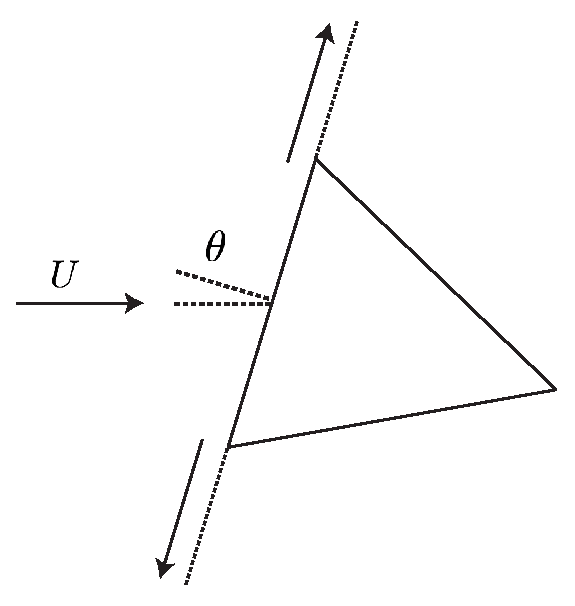
\includegraphics[width=0.25\unitlength]{./chapter-cross-sections/fnp/tri-sketch.eps}}         
      
      
   
 	\put(0.38,0.937){$\theta$}
 	%\put(0.52,0.74){$l$}
   

 	
 	 

     

  \end{picture}

 \caption{Illustration of the lines along which the flow velocity magnitudes have been extracted. The data have been extracted along a line starting from the separation points in the outward direction (shown with arrows) for the top and bottom surfaces.}
    \label{fig:tri-sketch}
\end{figure}


\begin{figure}
  \setlength{\unitlength}{\textwidth}

        \begin{picture}(1,1.1)(0,0.35)

      % % % Parkinson Data 
      \put(0.1,1.1){\includegraphics[width=0.75\unitlength]{./chapter-cross-sections/fnp/vel_prof-tri-4.eps}}
      \put(0.1,0.737){\includegraphics[width=0.75\unitlength]{./chapter-cross-sections/fnp/vel_prof-tri-16.eps}}
      \put(0.1,0.38){\includegraphics[width=0.75\unitlength]{./chapter-cross-sections/fnp/vel_prof-tri-21.eps}}
     
      
      



%      
    \put(0.21,1.41){\small(a)}
     \put(0.21,1.05){\small(b)}
     \put(0.21,0.69){\small(c)}
\put(0.1,0.95){$\displaystyle V_m$}
\put(0.1,1.3){$\displaystyle V_m$}
\put(0.1,0.56){$\displaystyle V_m$}
\put(0.34,0.35){Distance from the leading edge}

      
    \end{picture}

    \caption{Velocity magnitudes of the flow along a line parallel to the front surface spreading towards top (\solidrule) and bottom (\dashedrule) boundaries (figure \ref{fig:tri-sketch}). These two lines (for the top and bottom surfaces) start from the top and bottom leading edges of the triangular cross section. Data present (a) $\alpha=4^\circ$, (b) $\alpha=16^\circ$ \ and (c) $\alpha=21^\circ$.}
    \label{fig:surf_pres}
\end{figure}

 %vspace{10cm}


The maximum velocity magnitude in the top wall jet at $\theta= 4^{\circ}$ (figure \ref{fig:vel-profile} (a)) is higher than that in the corresponding bottom wall jet, leading to a lower pressure at the top edge. However, the velocity magnitude in the bottom wall jet becomes greater than that in the top wall jet at $\theta=16^{\circ}$. The difference between the top and bottom velocity magnitude in these wall jets tends to increase as $\theta$ is increased to $21^{\circ}$, where the velocity magnitude at the bottom is greater than at the top (figure \ref{fig:vel-profile} (c)). This effectively creates the pressure difference (according to the Bernoulli's principle ) shown in figure \ref{fig:surf_pres} (c), which leads to a positive \cy\ and results in a forcing which is in phase with the velocity of the body. 







%KASUN: Does the velocity go back to zero at 0 distance? Why not show
%the whole range of $V_m$?
%
%Also, pick a symbol for the distance rather than writing ``Distance
%from the trailing edge'', and show this symbol on the graph and the
%sketch.
%
%Also, you realise you have used $\alpha$ in the caption of angle of
%attack, but the rest of your thesis uses $\theta$?
%
%
%
%KASUN: I am not convinced by this. I can see that the magnitude of the upper jet increases with $\theta$, but the lower one seems almost unaffected. I can also see that the maximum of the upper jet first moves towards the surface, then away again. How does this fit with your basic Bernoulli argument?
%
%Why do you need profiles at all? Why can't you plot contours of velocity magnitude? In fact, you could also replace figure 3.4 with plots of pressure contours. Or keep what you have but add plots of contours. I think this whole section would also be stronger if you contrasted a low \ratio\ case (the triangle) with a high \ratio\ case (the square).
%
%Also, why does the dotted line change format between a and b?


\subsection{Mean streamlines}

The shear layers of the body can be visualised using the magnitude of the strain rate tensor The strain rate is directly proportional to the shear stress and so it will be high in the shear layers. Instantaneous flow-field data consists of vortex shedding on top of the shear layers. Hence, the flow-field data are time averaged over a vortex shedding cycle to filter out the vortex shedding . 

The strain rate tensor of the flow can be expressed as,

\begin{equation}
\varphi = \frac{1}{2}
\begin{bmatrix}
2\frac{\partial u}{\partial x} & \frac{\partial u}{\partial y} + \frac{\partial v}{\partial x} \\
\frac{\partial v}{\partial x} + \frac{\partial u}{\partial y} & 2\frac{\partial v}{\partial y} \\
\end{bmatrix}
\end{equation}

thus the magnitude of the strain rate tensor becomes,

\begin{equation}
|\varphi| = \frac{1}{2}\left(4\frac{\partial u}{\partial x}\frac{\partial v}{\partial y} + \left(\frac{\partial u}{\partial y} + \frac{\partial v}{\partial x}\right)^2\right)
\end{equation}.



\begin{figure}[!h]

  \setlength{\unitlength}{\textwidth}

  \begin{picture}(1,0.35)(0,0.725)

    \put(-0.01,0.76){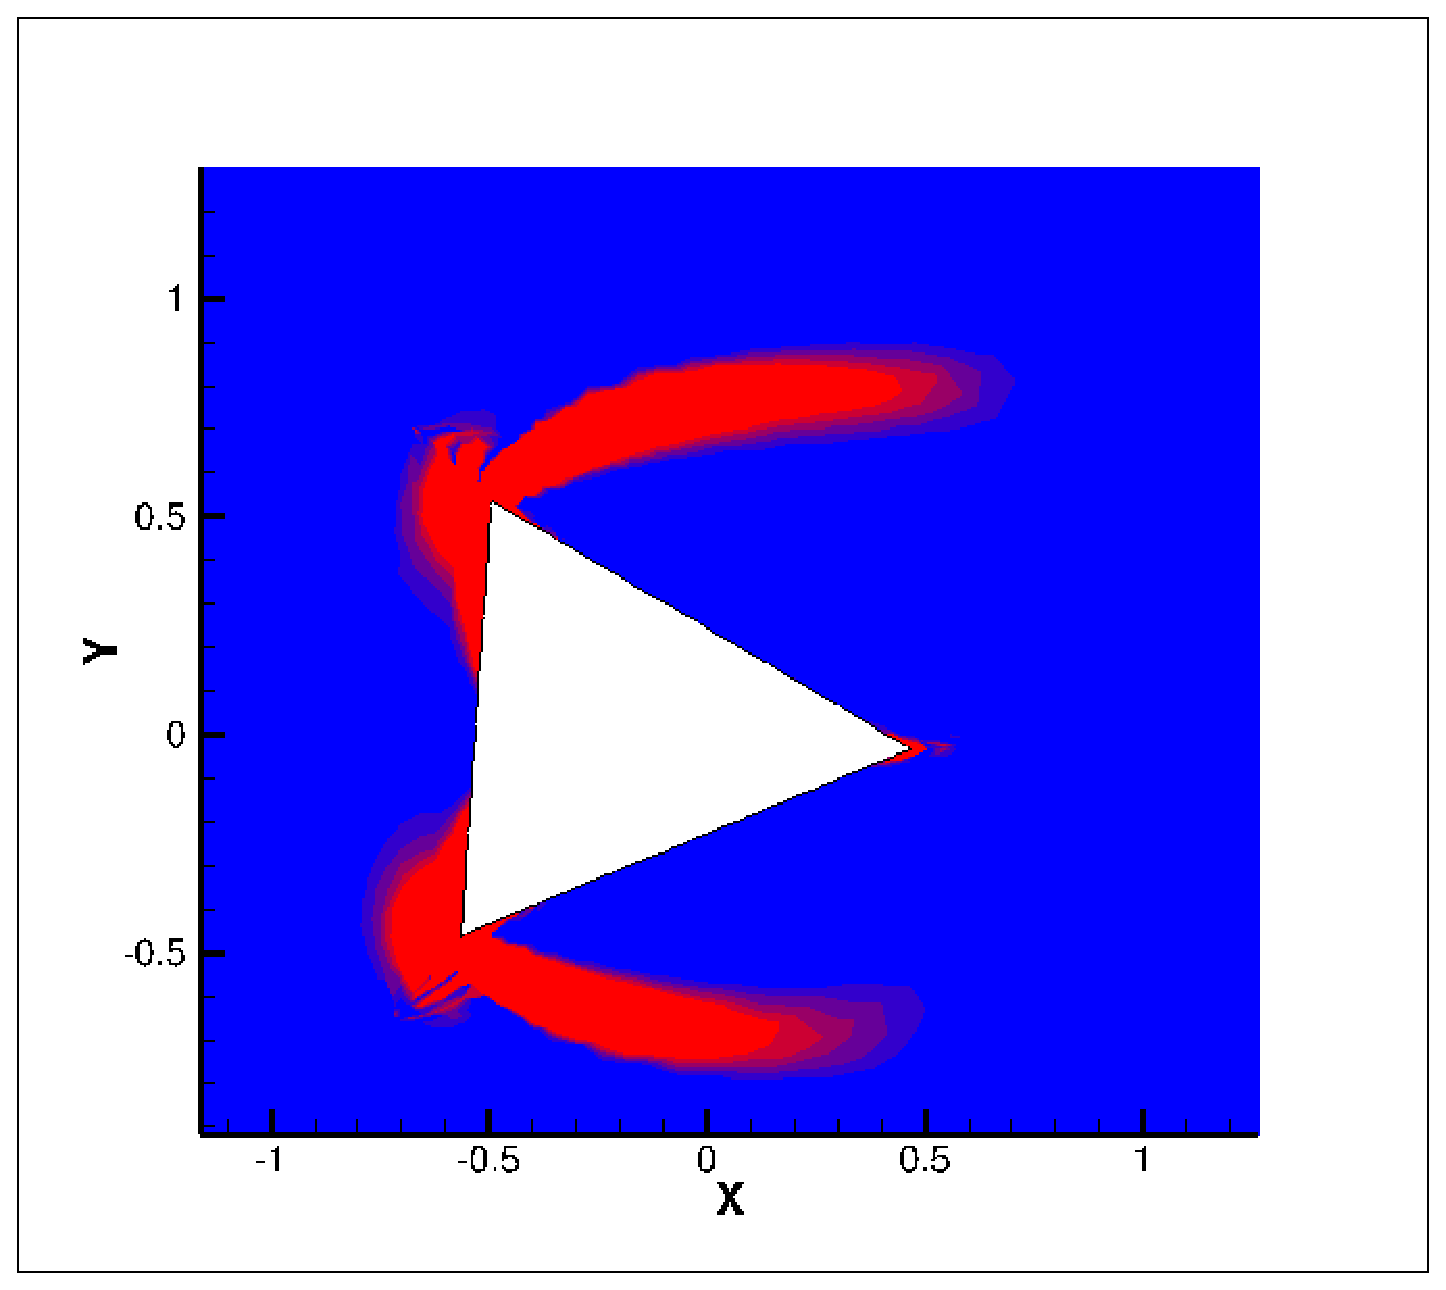
\includegraphics[width=0.33\unitlength]{./chapter-cross-sections/fnp/4.eps}}
    \put(0.335,0.76){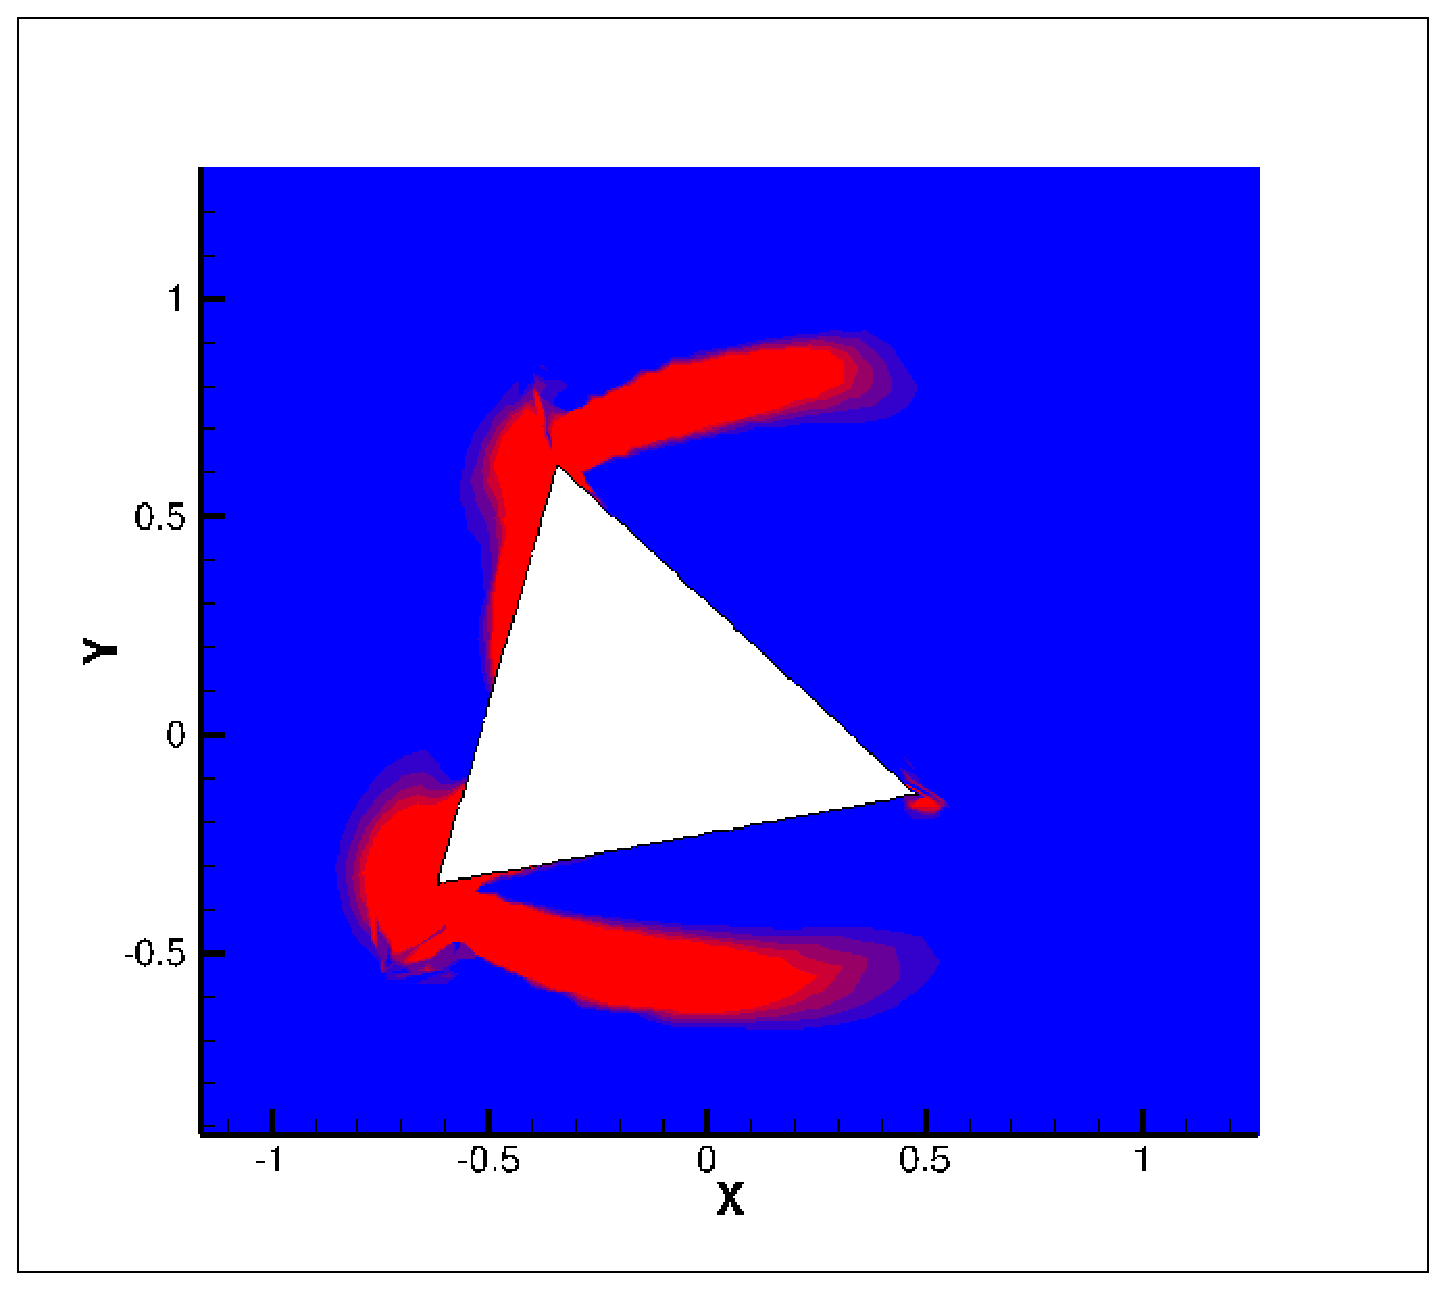
\includegraphics[width=0.33\unitlength]{./chapter-cross-sections/fnp/16.eps}}
    \put(0.68,0.76){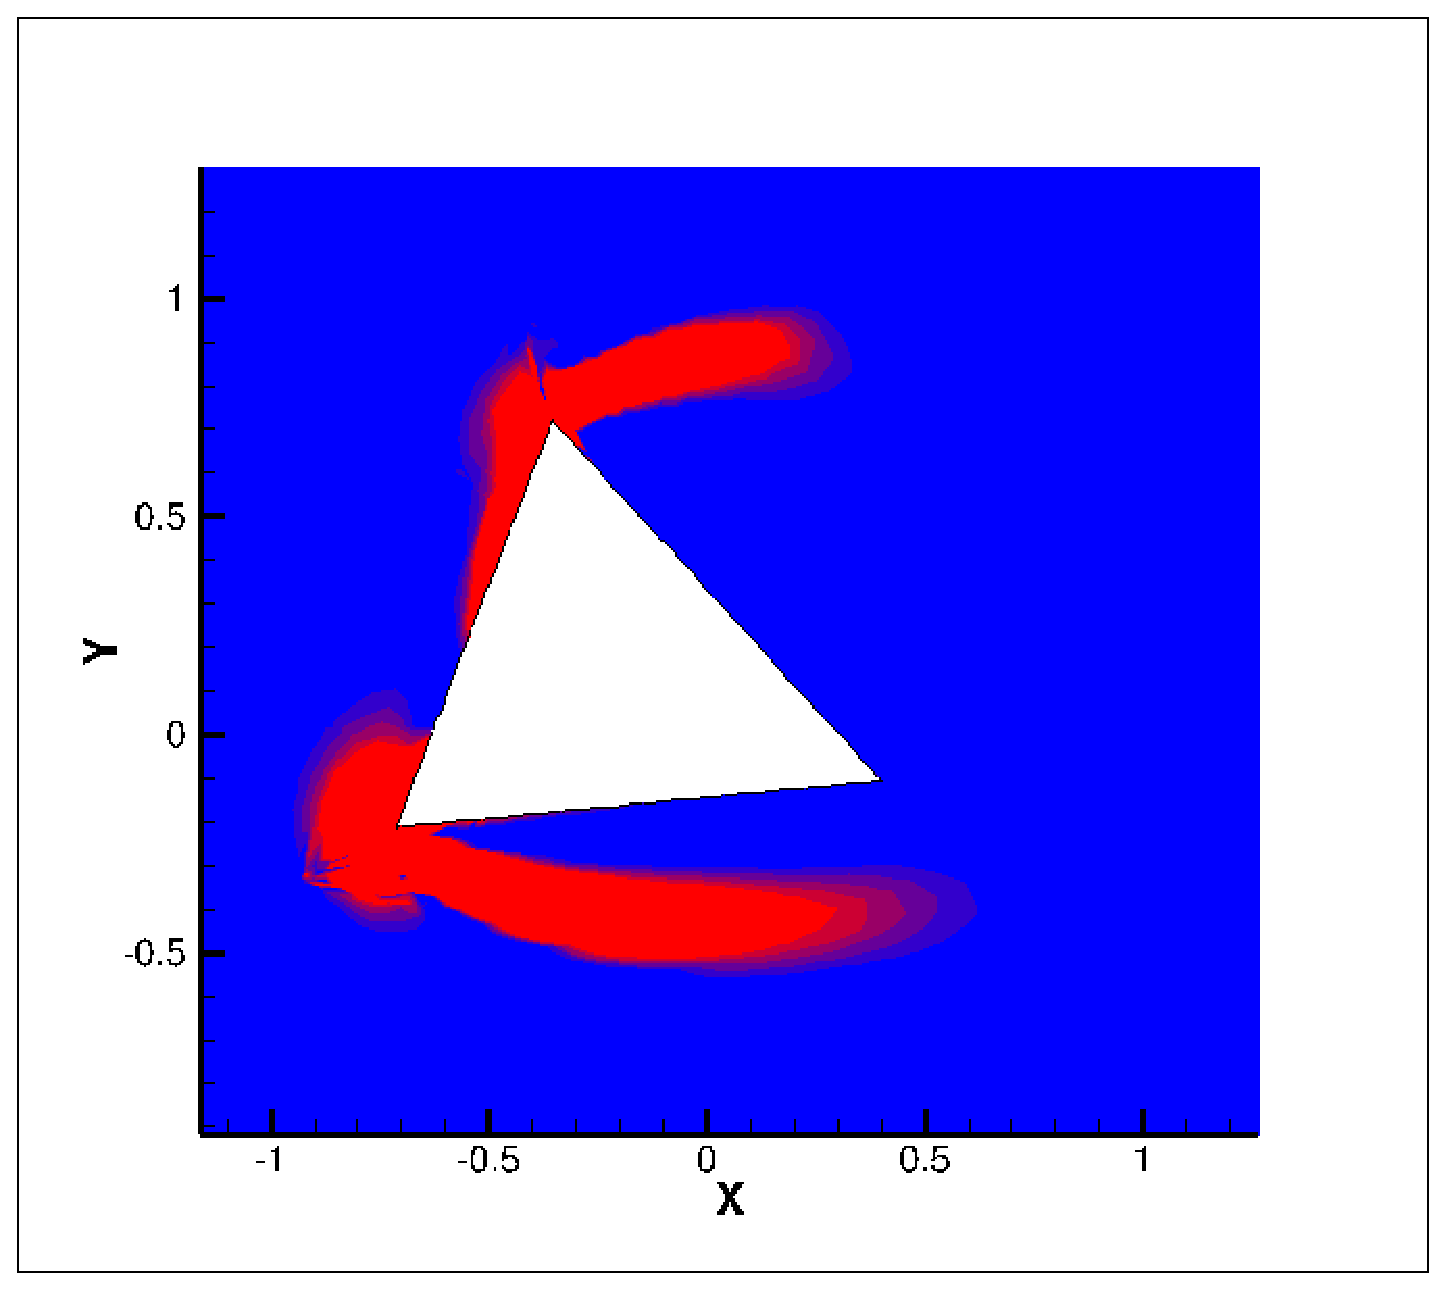
\includegraphics[width=0.33\unitlength]{./chapter-cross-sections/fnp/21.eps}}

   
    
    \put(0.0,0.735){(a)}    
    \put(0.34,0.735){(b)}
    \put(0.685,0.735){(c)}
  
  \end{picture}

  \caption{Contours of the magnitude of the shear strain rate of time averaged flow field on the  stationary isosceles triangle ($\ratio=0$) at $\reynoldsnumber=200$ at different incidence angles. (a) $4^{\circ}$ ( negative value of \cy\ that is further decreasing with increasing $\theta$), (b) $16^{\circ}$ ( negative value of \cy\ that is increasing with increasing $\theta$) and (c) $21^{\circ}$ (a significantly positive value of \cy). The bottom shear layer comes closer to the bottom wall and as the angle of incidence increases.}
  \label{fig:triangle-shear_layers}
\end{figure}




  



Contours of the magnitude of the strain rate tensor of the time averaged flow-field of the stationary isosceles triangle at  $\theta=4^{\circ}$, $\theta=16^{\circ}$ and $\theta=21^{\circ}$ are presented in figure \ref{fig:triangle-shear_layers}. Here, it can be observed that the proximity of the bottom shear layer increases as $\theta$ is increased from $4^{\circ}-21^{\circ}$. 


By comparing the pressure and the velocity plots together with the flow-field data, it is evident that there are two mechanisms governing the transverse forcing. The first mechanism is the pressure difference in each shear layer, created as a result of the uneven distribution of the flow created due to the profile and  positioning (angle of attack) of the geometry. This uneven distribution creates a different speed wall jet on either side, and a simple consideration of Bernoulli's equation suggests the higher speed jet will have a lower pressure. This forcing occur out of phase or in the opposite direction of the transverse velocity of the body, as the lower speed (higher pressure) jet is formed on the lower side of the body (when the body is travelling down). The second mechanism is the relative proximity of the top and bottom shear layers. Regardless of the pressure in each shear layer, that pressure will have a larger influence on the force on the body the closer the shear layer is to the body. So, there are two ways to manipulate the force from the shear layers; increase the pressure difference between the shear layers by increasing the difference between the flow in each shear layer (a ``streaming effect''); move the shear layers closer or further from the body (the ``proximity effect'').

Initially at $\theta= 4^{\circ}$ the streaming effect dominates. This can be observed comparing figures \ref{fig:triangle-shear_layers} (a) to (b) and (c). The  bottom shear layer is far from the body at $\theta= 4^{\circ}$, hence the proximity effect is low. This results in the negative \cy.   

As $\theta$ is increased first to $\theta=16^{\circ}$ and then to $21^{\circ}$, the proximity of the bottom shear layer to the wall of the body increases (figure \ref{fig:triangle-shear_layers} (b) and (c)), and thus the proximity effect becomes more dominant. At least for the $\theta = 21^{\circ}$ case, this creates the positive region of the \cy\ vs. $\theta$ curve.

% % % % % % % % % % % % % % % % % % % % % % % % % % % % % % % % % % % % % % % % % % % % % % %
\section{Fluid-structure interaction (DNS) results}
\label{sec:cross-sec-FSI-results}

\subsection{Mean power data}
\label{subsec:cross-sec-dns-mean-power}

 The main limitation of the QSS model as discussed in section \ref{sec:dns} is considering the induced transverse force $F_{y}$ as the sole driving force of the system, generated by the relative proximity of the shear layers (refer section \ref{subsec:c_y and shear layers}). However, it was concluded in chapter \ref{chap:pi_1_pi2} the QSS model provides good agreement between QSS and DNS for power at high \massstiff\ for the square cross section, even though the relative error increased as \massstiff\ decreased due to the significant influence of vortex shedding.


  A comparison study between QSS and DNS mean power was carried out on the different cross sections considered at high \massstiff\ (i.e.$\massstiff=1000$) and presented in figure \ref{fig:DNS-power}.
\begin{figure} [htb]
  \setlength{\unitlength}{\textwidth}

        \begin{picture}(1,0.46)(0,0.4)

      \put(0.1,0.45){\includegraphics[width=0.75\unitlength]{./chapter-cross-sections/fnp/qss-dns-mean-power.eps}}
      
%       \put(0.07,0.95){$\displaystyle\frac{V}{D}$}
%       \put(0.07,1.3){$\displaystyle\frac{A}{D}$}
       \put(0.06,0.68){$\displaystyle\frac{P_{m}}{\rho \mathcal{A}U^3 }$}
%       \put(0.5,0.4){$\massdamp$}
       \put(0.5,0.42){$\displaystyle\ratio$}
    
    \end{picture}

  % \caption{Comparison of maximum power between QSS and DNS data obtained using 3 point local quadratic curve fitting.The error was obtained using Eq:\ref{eqn:error_calculation}}
    \caption{Comparison of the maximum power obtained using DNS ($\displaystyle\bullet$) and the QSS ($\times$) model as a function of \ratio. Data obtained at $\massstiff=1000$ ($\mstar=201.3$) and $\reynoldsnumber=200$. Similar trends are present for both QSS and DNS data. A significant reduction in power could be observed as $\ratio \rightarrow 1$}
    \label{fig:DNS-power}
\end{figure}

 %vspace{10cm}

Both  DNS and QSS mean power data (figure \ref{fig:DNS-power}) show similar trends. The maximum mean extracted power increases as \ratio\ is decreased. These trends provide a reinforcement to the hypothesis of attaining a higher power output through inhibition of the shear layer reattachment.   

However, a significant error (calculated using equation \ref{eqn:error_calculation}) between QSS and DNS power could be observed as \ratio\ decreases. The quantified errors presented in figure \ref{fig:error-hybrid} shows an almost linear increase in the $\%$ error as $\ratio \rightarrow 0.25$, with a maximum error of $35\%$.

\begin{figure}
  \setlength{\unitlength}{\textwidth}

        \begin{picture}(1,0.4)(0,0.4)

      \put(0.1,0.45){\includegraphics[width=0.75\unitlength]{./chapter-cross-sections/fnp/qss-dns-pow-erroe.eps}}
      
%       \put(0.07,0.95){$\displaystyle\frac{V}{D}$}
%       \put(0.07,1.3){$\displaystyle\frac{A}{D}$}
       \put(0.08,0.58){\rotatebox{90}{\%   error}}
%       \put(0.5,0.4){$\massdamp$}
       \put(0.5,0.4){$\displaystyle\ratio$}
    \end{picture}

  % \caption{Comparison of maximum power between QSS and DNS data obtained using 3 point local quadratic curve fitting.The error was obtained using Eq:\ref{eqn:error_calculation}}
    \caption{The percentage error calculated using \ref{eqn:error_calculation} between the maximum power obtained using DNS data and predicted by QSS model as a function of \ratio. The error reduces significantly as $\ratio \rightarrow 1$}
    \label{fig:error-hybrid}
\end{figure}

 %vspace{10cm}

\subsection{Flow-field data}

As a significant discrepancy between the QSS and DNS data was observed, further investigations were conducted in order to identify the cause of this error. 

The QSS model assumes that the flow is quasi-static, meaning the instantaneous flow of the oscillating body at a particular induced angle $\theta$, is similar to that of a stationary body at the same induced angle. Thus, stream traces of the flow around the oscillatory body at selected instants of a single galloping cycle were compared against the stream traces of a similar stationary cross section at the induced angles produced at the considered points of the galloping cycle. The chosen cross section to perform this task was $\ratio=0.25$ at $\massdamp=0.26$ which provided the maximum mean power among all cases considered. Three points of a galloping cycle was considered. These points corresponded to key instants of the velocity signal. The points considered  were point 1 where $\dot{y}$ is maximum, point 2 where $\dot{y}$ is close to zero with a negative gradient and point 3 where $\dot{y}$ is close to zero with a positive gradient. An illustration of these points is presented in figure \ref{fig:FSI_sketch}.

It should be recalled that the QSS model assumes that only the long-time forces are important; the fluctuation in time at the frequency of the vortex shedding is assumed to play no role. Therefore, both stationary and the instantaneous oscillatory flow data were time averaged over a length of time equal to one vortex shedding cycle in order to filter the vortex shedding and have an estimate of the mean flow.   

% !TeX spellcheck = en_GB
\begin{figure}[!htb]
  \setlength{\unitlength}{\textwidth}

        \begin{picture}(1,0.4)(-0.02,0)

 
      
      \put(0.08,0.02){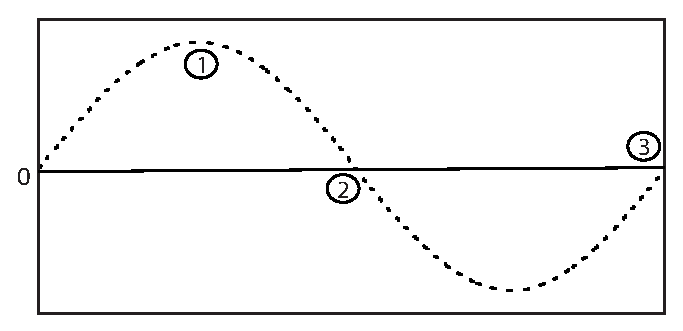
\includegraphics[width=0.75\unitlength]{./chapter-cross-sections/fnp/fsi_flow_sketch.eps}}

      %\put(0.46,0.00){\massdamp}
      
      
     
       %\put(0.03,0.235){$\displaystyle\frac{P_{m}}{\rho \mathcal{A}U^3 }$}
      

      %\put(0.095,0.218){\small(a)}
      %\put(0.565,0.218){\small(b)}
      
    \end{picture}

  \caption{}
    \label{fig:power_curves}
\end{figure}

 %vspace{10cm}



Figure \ref{fig:flow_field_FSI} shows the time averaged stream functions for points 1, 2 and 3 and the stationary time averaged stream traces of the corresponding induced angles. The time-averaging was carried out over a period of vortex shedding in oder to filter the effects of vortex shedding. Comparison between FSI and stationary data at point 1, where the transverse velocity is at its maximum, (Figure \ref{fig:flow_field_FSI} (a) and (b)) shows a significant difference of the stream functions. 

\begin{figure}[htbp]
  \setlength{\unitlength}{\textwidth}

  \begin{picture}(1,1.19)(0,0)
    % % %90
      % % % Parkinson Data 
      \put(0.005,0.8){\includegraphics[width=0.4\unitlength]{./chapter-cross-sections/fnp/{fsi-0.25-1}.eps}}
      \put(0.005,0.4){\includegraphics[width=0.4\unitlength]{./chapter-cross-sections/fnp/{fsi-0.25-2}.eps}}
      \put(0.005,0.0){\includegraphics[width=0.4\unitlength]{./chapter-cross-sections/fnp/{fsi-0.25-3}.eps}}

      
      
      \put(0.505,0.8){\includegraphics[width=0.4\unitlength]{./chapter-cross-sections/fnp/{qss-0.25-1}.eps}}
      \put(0.505,0.4){\includegraphics[width=0.4\unitlength]{./chapter-cross-sections/fnp/{qss-0.25-3}.eps}}
      \put(0.505,0.0){\includegraphics[width=0.4\unitlength]{./chapter-cross-sections/fnp/{qss-0.25-3}.eps}} 
      
      
%      \put(0.23,0.00){ $\displaystyle\frac{c}{\rho\mathcal{A}U}$}
%      \put(0.73,0.00){ $\displaystyle\frac{c}{\rho\mathcal{A}U}$}


      
      \put(0.01,1.125){\small(a)}
      \put(0.510,1.125){\small(b)}
      \put(0.01,0.725){\small(c)}
      \put(0.510,0.725){\small(d)}
      \put(0.01,0.33){\small(e)}
      \put(0.510,0.33){\small(f)}
      
   
   
      

  \end{picture}

  \caption{Time averaged stream functions of stationary and oscillating flow-fields of the hybrid cross section ($\ratio=0.25$), averaged over a vortex shedding cycle. (a), (c) and (e) are the averaged stream functions of the oscillating case at $\frac{tU}{D}=2295.763$ (point 1), $\frac{tU}{D}=2305.897$ (point 2) and $\frac{tU}{D}=2325.870$ (point 3) . (b), (d) and (f) are the stream functions of the flow field of the stationary body corresponding to the induced angles of (a), (c) and (e).}  
  \label{fig:flow_field_FSI}
\end{figure}

In contrast, at point 2 and 3 the stream functions at the leading edge of the FSI simulations are similar to those of the stationary simulations. At point 2 both the FSI (figure \ref{fig:flow_field_FSI} (b)) and stationary  case (figure \ref{fig:flow_field_FSI} (c)) show similar flow behaviour until separation. A single circulation bubble at the top is formed in the FSI case where a symmetrical formation of the circulation bubbles could be observed in the stationary case. A similar behaviour of the stream functions could be observed between point 3 for FSI (figure \ref{fig:flow_field_FSI} (d)) and stationary (figure \ref{fig:flow_field_FSI} (e)) cases. 

According to the assumptions of the QSS theory the flow-fields between the stationary and FSI cases at points 2 and 3 should be approximately identical as the induced velocities are zero and therefore the induced angles are zero. However, the observations on the corresponding FSI cases show a significant difference, indicating a significant deviation from the quasi-steady assumption.

Thus, from the analysis of the flow data it is clear that the  QSS predictions deviates significantly for mean power predictions at decreasing \ratio, as a result of the flow not being quasi-static. Thus, this violates the assumption of considering the time averaged fluid forces as the inputs of the oscillatory system creating a significant discrepancy between QSS and DNS mean power.    

 However, the QSS model does provide similar trends as the DNS predictions and therefore, can be used as a preliminary design and research tool to obtain data and conclusions to produce efficient galloping energy extraction systems. 
  
 \section{Design considerations for a galloping energy extraction system through inhibition of shear layer reattachment.}
 \label{subsec:design-considerations-cross-section}
 
 From the QSS and DNS results it is clear that inhibition of the shear layer reattachment  leads to higher energy output. However, it is to be noted that even though a higher power output could be obtained through inhibition of the shear layer reattachment, a region of adverse power transfer (body-to-fluid)  will develop as \ratio\ decreases. This can be observed through the negative region present in the $\cy$ curves beyond $\ratio\leq0.25$. As this negative region develops the maximum extracted power reduces,which can be observed in the power curves (figure \ref{fig:power_curves}) where the maximum power at $\ratio=0$ is less than $\ratio=0.25$.
 
 This fact leads to one important design consideration for an optimum cross section. The optimal design would be a trade off between large positive values of \cy\ occurring at high angles of attack where significant power could be generated and the negative regions of \cy\ where the power transfer occurs in the opposite direction. \citet{Barrero-Gil2010a} concluded that the first coefficient $a_1$ should satisfy  $a_1>0$ in order to obtain good operation of an energy harvesting system, where it is furthermore explained in detailed using the QSS model together with direct numerical simulations for FSI cases. The conclusion of Barrero-Gil could be considered as somewhat simplistic as cases of higher power output where $a_1 < 0$ can be observed in figure \ref{fig:power_curves}. Thus, a more detailed statement to compliment Barrero-Gil is to obtain a cross section which produces a \cy\ vs. $\theta$ curve with optimum balance between negative and positive regions.  
 
  As further consideration for future research, DNS and QSS work at $0<\ratio<0.25$ could be carried out to find the optimum ratio of $\ratio$ to obtain a maximum power output. Moreover, further work could be carried out to find ways to reduce the negative portion of the $\cy$ curve by applying modifications to the cross section which can result in further optimisation of the geometry.
 
 \section{Summary} 
 \label{sec:summary-diff-cross-sec}
 
 The primary objective of the work presented in this chapter was to test the hypothesis that higher power output could be obtained by inhibition of shear layer reattachment. This was done by incrementally tapering off the top and bottom sides of the trailing edges of the square cross section. A negative region in the $\cy$ vs. $\theta$ curve was observed for $\ratio<0.25$. This region resulted in a power loss in a certain portion of the galloping cycle as the driving force $F_y$ and the velocity $\dot{y}$ were in opposite directions.
 
 The mean power versus \massdamp\ curves showed an increase in maximum power as $\ratio$ was decreased until $\ratio=0.25$. At $\ratio=0$,  ($\displaystyle\frac{P_{m}}{\rho \mathcal{A}U^3}=0.0304$ at $\massdamp=0.021$) the maximum power was less than at $\ratio=0.25$ ($\displaystyle\frac{P_{m}}{\rho \mathcal{A}U^3}=0.04$ at $\massdamp=0.028$), although the peak value of both the induced angle and \cy\ were greater in $\ratio=0$ compared to $\ratio=0.25$. Further analysis of the \cy\ curve revealed that the negative region of $\ratio=0$  was greater than that of $\ratio=0.25$, hence resulting in a lower maximum power output. 
 
 The surface pressure plots and the velocity magnitude profiles at the starting points of the wall jets revealed  that there are two mechanisms governing the transverse forcing. The first mechanism is the pressure difference in each shear layer, or the ``streaming effect''. The second mechanism was the relative proximity of the top and bottom shear layers, or the ``proximity effect''.

 Initially at $\theta= 4^{\circ}$ the streaming effect dominated resulting the negative \cy. As $\theta$ increased from  $\theta= 16^{\circ}$ to  $\theta= 21^{\circ}$ the proximity effect started dominating resulting in a positive \cy.
 
Comparison of the QSS and DNS predictions of maximum power showed similar trends. The maximum power increased as \ratio\  decreased supporting the hypothesis of attaining higher power output through inhibition of shear layer reattachment. However, a significant error between the QSS and FSI simulations were observed as \ratio\ was reduced. 
 
Further investigations carried out using time averaged flow data concluded that the mean flow of FSI simulations had significant deviations from the DNS stationary simulations carried out at corresponding induced angles. This shows that the flow is essentially not quasi-static, violating the primary assumption of considering $F_y$ as the sole driving force of the system. Yet, the QSS model can be used as a tool to obtain initial approximations to design galloping energy harvesting systems as QSS data produced similar trends as the FSI simulations.
 
In order to obtain an efficient galloping energy harvesting system through inhibition of shear layer reattachment, one key design consideration is to obtain a cross section which has the optimum balance between the negative and positive regions of the $\cy$ vs. $\theta$ curve. Inhibition of  the shear layer reattachment through tapering of the trailing edge leads to higher power. However, as it approaches a triangle, a negative region of $\cy$ emerges in the \cy\ vs. $\theta$ curve which leads to adverse power transfer. This region keeps increasing between $0\leq\ratio\leq0.25$. Thus as a result an optimum \ratio\ should be obtained in order to get a balance between the negative and positive regions which leads to an optimal galloping energy harvesting system. 
 
 As for future research this method of attaining high power through inhibition of shear layer reattachment can be further developed by conducting more detailed investigations into the geometry to find ways to reduce the adverse power transfer which will lead to further increases in power output.
